\documentclass[10pt]{article}

\usepackage[utf8]{inputenc}
\usepackage[french]{babel}
\usepackage[T1]{fontenc}
\usepackage{lmodern}
\usepackage{hyperref}
\usepackage{amsthm}
\usepackage{amscd}
\usepackage{mathtools}
\usepackage{amssymb}
\mathtoolsset{showonlyrefs=true}
\usepackage{fullpage}
\usepackage{graphicx}

%Il faut qu’on écrive une page ou deux par contre, pour expliquer le projet. En gros un titre,   
\title{Ce que l'étude d'impact ne dit pas}

\author{Bruno Scherrer \and Michaël Baudin}


\begin{document}

\maketitle

\tableofcontents

\section{Résumé}

Le 24 Janvier 2020, le gouvernement a rendu public une 
étude d'impact ayant pour objectif de présenter le projet 
de loi instituant le système universel de retraites. 
L'objectif du présent texte est de permettre de comprendre 
l'influence de cette réforme sur l'équilibre financier macro-économique 
du système de retraite. 
Nous montrons pourquoi les simulations montrent que l'âge de départ à la 
retraite augmente et que le niveau des pensions diminue, contrairement à ce que laisse 
penser l'étude d'impact. 
Ainsi, l'étude d'impact ne présente pas de résultat techniquement faux : 
elle se contente de dissimuler l'effet de la réforme \emph{par omission}, 
laissant penser ce qu'elle ne dit, en fait, pas. 

%%%%%%%%%%%%%%%%%%%%%%%%%%%%%%%%%%%%%%%%%%%%%%

\section{Modèle du simulateur officiel du COR}

\subsection{Présentation du modèle}

Dans le but de pouvoir comprendre l'influence des changements indiqués par 
l'étude d'impact, nous souhaiterions pouvoir utiliser le simulateur du COR 
(\url{https://www.cor-retraites.fr/simulateur}). 
Comme nous allons le voir, l'exercice de reproduction des résultats 
de l'étude d'impact révèle les intentions de ses auteurs. 

Ce simulateur tient compte de deux variables permettant de définir un scénario :
\begin{itemize}
\item le taux de hausse des salaires : +1\%, +1.3\%, +1.5\%, +1.8\%, 
\item le taux de chômage : 4.5\%, 7\%, 10\%.
\end{itemize}

Les scénarios de base sont les suivants :
\begin{itemize}
\item taux de chômage : 7\%, taux de hausse des salaires : +1\%, 
\item taux de chômage : 7\%, taux de hausse des salaires : +1.3\% - scénario "central", 
\item taux de chômage : 7\%, taux de hausse des salaires : +1.5\%, 
\item taux de chômage : 7\%, taux de hausse des salaires : +1.8\%.
\end{itemize}
De plus, deux scénarios complémentaires sont présentés :
\begin{itemize}
\item un scénario "pessimiste" : taux de chômage : 10\%, taux de hausse des salaires : +1\%, 
\item un scénario "optimiste" : taux de chômage : 4.5\%, taux de hausse des salaires : +1.8\%. 
\end{itemize}

Les rapports du COR s'appuient la plupart du temps sur le taux 
de chômage de 7\% et prennent en compte les différents taux de hausse 
des salaires de +1\% à +1.8\%. 
Au contraire, l'étude d'impact ne présente généralement qu'une seule 
courbe, correspondant au scénario central avec un taux de chômage de 7\% et une hausse des 
salaires de +1.3\%. 
Ainsi, on ne peut pas connaître l'influence de ce paramètre sur les calculs 
de l'étude d'impact. 
Cela constitue un premier étonnement. 

Une fois le scénario choisi dans le simulateur du COR, 
l'utilisateur doit ajuster trois leviers : 
\begin{itemize}
\item l'âge de départ à la retraite, 
\item le taux de cotisation, 
\item le niveau des pensions par rapport aux salaires. 
\end{itemize}

En sortie, le simulateur du COR calcule :
\begin{itemize}
\item la situation financière du système de retraites, 
\item le niveau de vie des retraités, 
\item la durée de vie passée à la retraite. 
\end{itemize}

On peut utiliser ce simulateur de différentes manières, mais la 
logique qui a dominé dans le passé a consisté à se fixer un objectif 
de niveau de vie des retraités, puis à augmenter l'âge de départ ou 
le taux de cotisations, tout en élevant progressivement le niveau des pensions. 

%%%%%%%%%%%%%%%%%%%%%%%%%%%%%%%%%%%%%%%%%%%%%%

\subsection{Difficultés dans l'étude d'impact}

Reproduire les simulations de l'étude d'impact avec le simulateur du COR 
est donc impossible à priori. 
D'une part, le simulateur ne présente pas le niveau de dépenses du système 
de retraites. 
Etant donné le niveau de dépenses actuel, égal à 13.6\% en 2020, 
l'objectif du gouvernement est d'abaisser ce niveau de dépenses 
en direction du niveau moyen européen. 
D'autre part, le simulateur permet d'observer le solde financier du système de retraites, 
mais ne permet pas facilement d'imposer l'équilibre, c'est à dire un solde nul. 
Or cet équilibre financier est l'objet du projet de loi organique de la réforme 
des retraites. 

C'est pourquoi une inversion mathématique est nécessaire pour pouvoir reproduire 
les résultats de l'étude d'impact. 
C'est la raison pour laquelle nous avons développé un simulateur Open Source 
(\url{https://github.com/brunoscherrer/retraites}) fondé sur les mêmes équations mathématiques 
que le simulateur du COR, mais dont nous avons inversé les relations pour 
pouvoir imposer les paramètres pris en compte dans l'étude d'impact. 

Une difficulté apparaît lorsqu'on fait les calculs : 
l'étude d'impact s'arrête en 2050, alors que les rapports du COR 
se projettent jusqu'en 2070. 
C'est un second étonnement. 
C'est la raison pour laquelle nous sommes contraints de faire des 
hypothèses sur les variables imposées entre 2050 et 2070. 

%%%%%%%%%%%%%%%%%%%%%%%%%%%%%%%%%%%%%%%%%%%%%%

\subsection{Différence entre ensemble de la population et génération}

Dans ce paragraphe, nous détaillons la différence entre 
l'ensemble de la population à une date donnée et la génération d'une année 
de naissance donnée. 

En effet, lorsqu'on cherche à reproduire les simulation de l'étude d'impact, nous 
avons besoin de données relatives à l'année de départ en retraite. 
Une difficulté importante vient du fait que les graphiques de l'étude 
d'impact sont réalisés, au contraire, par génération. 
Dans l'étude d'impact, une génération correspond à l'ensemble des personnes 
nées la même année. 

La figure \ref{fig-trajectoire-vie} présente les générations des années 1940 
à 2010 environ, pour lesquelles nous avons utilisé les hypothèses du COR (Juin 2019).
Nous avons représenté par un point bleu l'année de naissance, par un point 
vert l'année de départ à la retraite et par un point rouge l'année de la 
mort. 

Observons tout d'abord que l'espérance de vie à 60 ans est supérieure à la 
différence entre l'espérance de vie à la naissance et 60 ans :
$$
E.V.(\textrm{60 ans}) \geq E.V.(\textrm{naissance}) - 60.
$$
Pour calculer l'année de mort, nous avons utilisé l'espérance de vie à 60 ans 
fournie par le COR. 
Observons que notre calcul est une approximation puisque nous aurions pu utiliser 
l'espérance de vie à la naissance. 
Toutefois, cela aurait mal reflété la durée de vie à la retraite pour ceux 
d'entre nous qui ont la chance de vivre jusqu'à cette date. 

\begin{figure}
\begin{center}
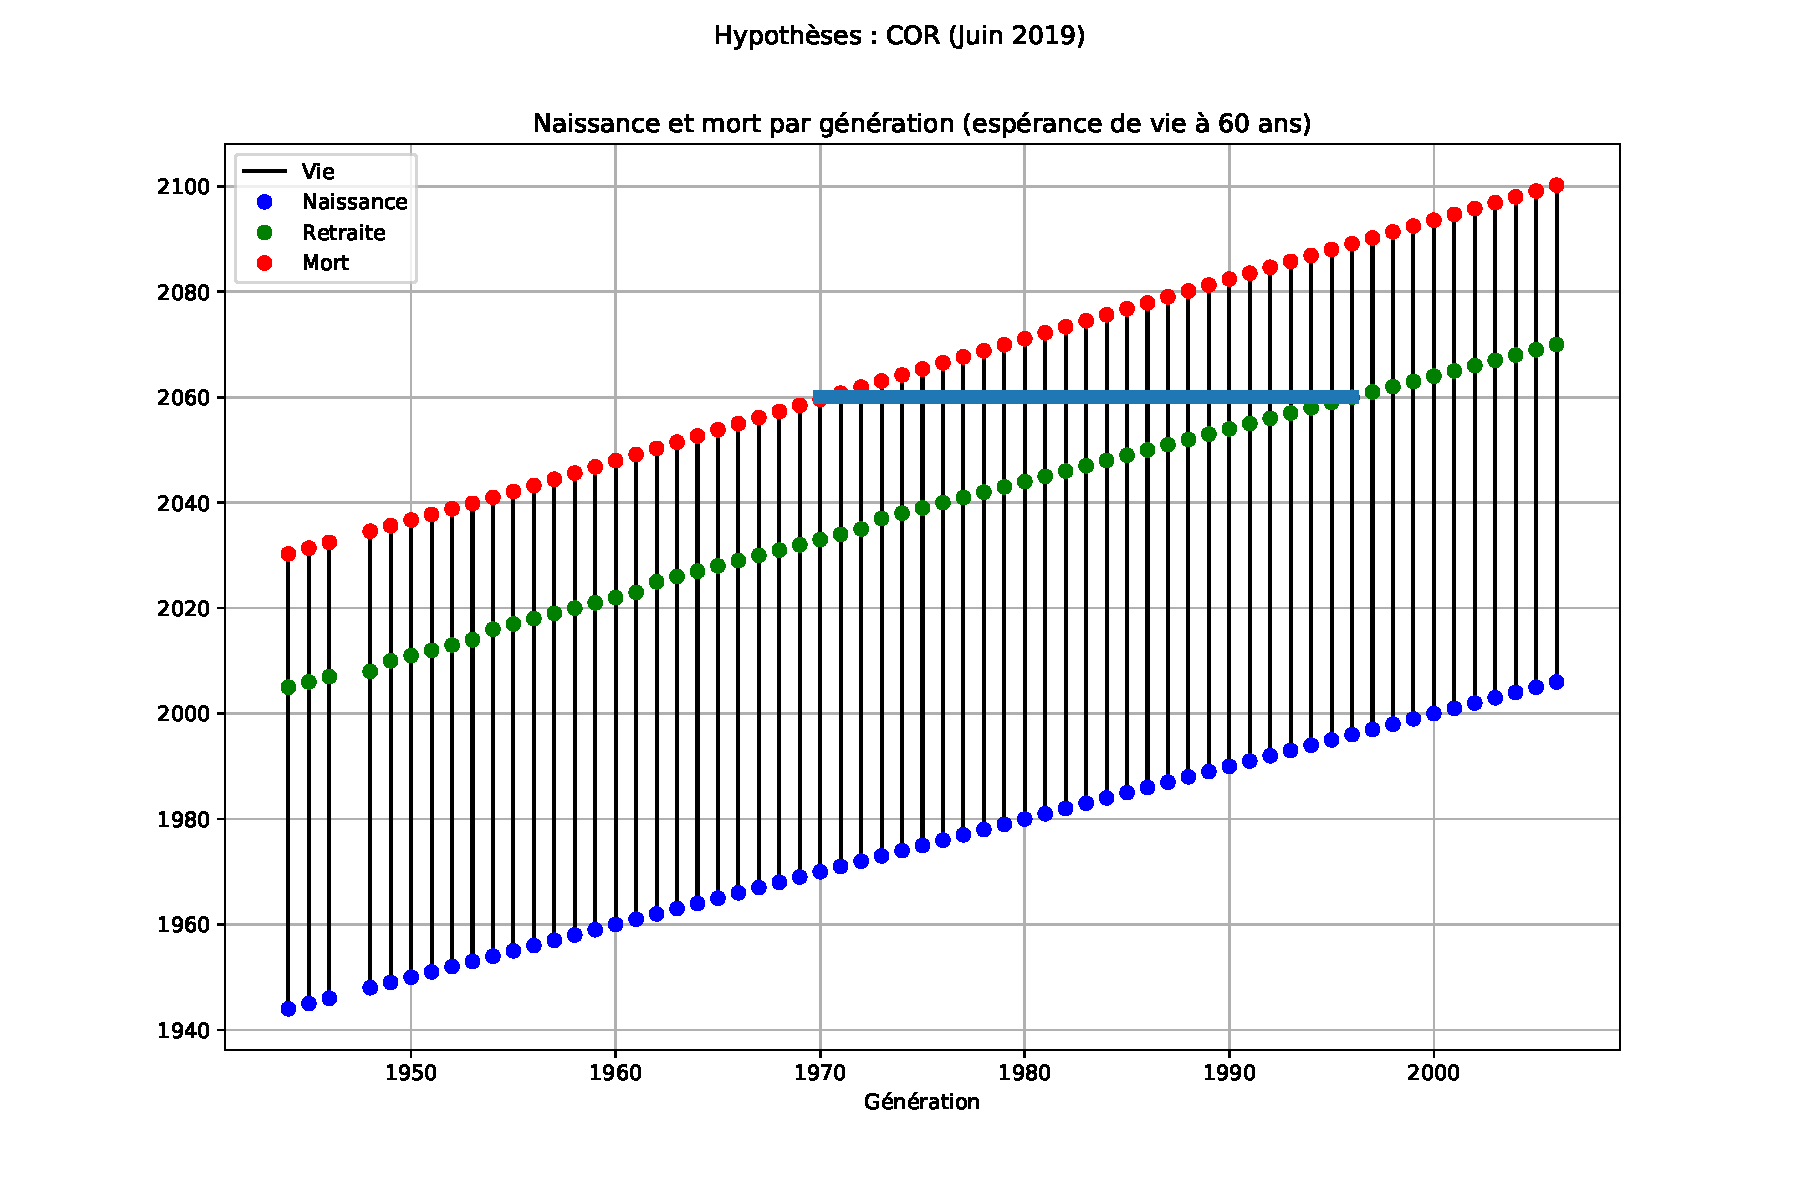
\includegraphics[width=0.9\textwidth]{Simulation-generation-vs-annee.pdf}
\end{center}
\caption{Trajectoire de vie de la naissance à la mort avec 
les hypothèses du COR (Juin 2019). 
Les générations dont l'individu moyen est en retraite en 2060 
sont les générations 1970 à 1996. }
\label{fig-trajectoire-vie}
\end{figure}

Pour une année donnée, plusieurs générations se côtoient au sein de la population des retraités. 
Pour le voir, on peut tracer la ligne horizontale correspondant à chaque année et observer les générations retraitées dont l'individu moyen est en vie à cette date. 
Par exemple, en 2060, l'individu moyen de la génération 1970 (et des générations précédentes) est mort tandis que que les générations nées après 1996 ne sont pas encore à la retraite. 
Par conséquent, les générations dont l'individu moyen est en retraite en 2060 sont les générations 1970 à 1996. 

Ainsi, lorsque nous souhaitons inférer le comportement de l'ensemble de la 
population des retraités lors d'une année donnée, nous ne devrions pas, en toute 
rigueur, utiliser les données d'une génération seulement. 

%%%%%%%%%%%%%%%%%%%%%%%%%%%%%%%%%%%%%%%%%%%%%%

\section{Hypothèses de calcul}

Notre calcul se fonde sur trois variables d'entrée :
\begin{itemize}
\item la situation financière du système de retraites, 
\item les dépenses du système de retraites, 
\item l'âge de départ à la retraite. 
\end{itemize}

L'ordre des priorités compte. 
L'équilibre financier prime sur tout le reste. 
Puis vient la diminution des dépenses par rapport à leur niveau actuel. 
L'âge de départ à la retraite doit donc augmenter. 
Dans la suite du texte, nous allons préciser quantitativement 
les évolutions prévues de chaque paramètre. 

%%%%%%%%%%%%%%%%%%%%%%%%%%%%%%%%%%%%%%%%%%%%%%

\subsection{L'équilibre financier}

L'équilibre financier est certainement la variable 
la plus facile à ajuster. 

L'étude d'impact, page 180, présente une analyse du solde financier du système de retraite 
avant et après réforme.
La figure \ref{fig-solde-etude-impact} est extraite de l'étude d'impact 
(graphique 63 page 180). 

\begin{figure}
\begin{center}
\includegraphics[width=0.9\textwidth]{../Figures-Etude-Impact/EtudeImpact-Graphique-63-situation-financiere.png}
\end{center}
\caption{Solde financier avant et après réforme d'après l'étude d'impact.}
\label{fig-solde-etude-impact}
\end{figure}

Le texte précise la trajectoire du "système universel de retraites" (SUR) : 
"Compte tenu des hypothèses décrites plus haut 
et en y ajoutant une mesure conventionnelle de redressement à court 
terme afin d’être à l’équilibre en 2027, le graphique ci-après présente 
la trajectoire du solde du SUR en la comparant à la trajectoire 
contrefactuelle (hors réforme) à l’horizon 2050."

C'est pourquoi nous devons considérer un solde financier :
\begin{itemize}
\item inchangé avant 2020,
\item linéairement croissant jusqu'à un solde nul en 2027,
\item puis nul ensuite.
\end{itemize}

Nous avons imposé ce solde financier dans notre propre simulateur. 
Les résultats que nous obtenons sont présentés dans la figure \ref{fig-solde-simulation}. 

\begin{figure}
\begin{center}
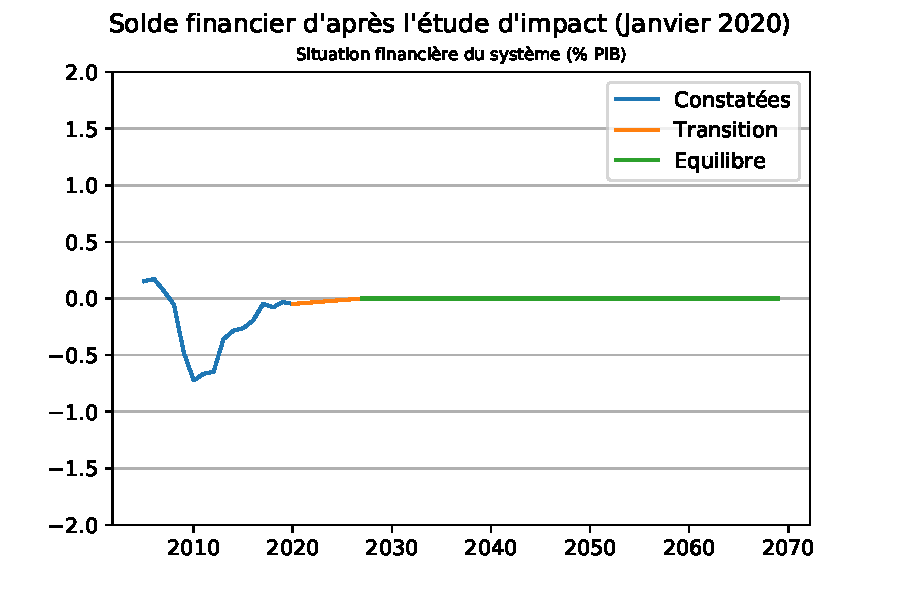
\includegraphics[width=0.7\textwidth]{Simulation-Solde-Financier.pdf}
\end{center}
\caption{Solde financier dans notre simulation de la réforme des retraites.}
\label{fig-solde-simulation}
\end{figure}

Insistons sur le fait que le système doit être à 
l'équilibre financier \emph{quelque soit la 
conjoncture économique}. 

%%%%%%%%%%%%%%%%%%%%%%%%%%%%%%%%%%%%%%%%%%%%%%

\subsection{Les dépenses de retraite}

L'étude d'impact, page 174, présente une analyse du niveau de dépenses 
en \% de PIB : "Ce taux est plus élevé que ce qu’on observe dans 
les autres pays européens. Les prestations de vieillesse-survie 
(correspondant au champ comparable internationalement, plus 
large que les dépenses du seul système de retraite) représentent 
14,4 \% du PIB en France, contre 12,6 \% du PIB dans l’UE-15 et 12,3 \% dans l’UE-28."
On comprend donc que l'objectif est de se rapprocher de la moyenne européenne. 

Dans le tableau 39 de l'étude d'impact, page 176, nous observons les valeurs numériques de la trajectoire de dépenses du système universel de retraites. 
Elles sont présentées dans la figure \ref{fig-depenses-etude-impact}.

\begin{figure}
\begin{center}
\includegraphics[width=0.9\textwidth]{../Figures-Etude-Impact/EtudeImpact-Tableau-39-Depenses-SUR.png}
\end{center}
\caption{Dépenses dans l'étude d'impact.}
\label{fig-depenses-etude-impact}
\end{figure}

Pour comparaison, la figure \ref{fig-depenses-UE-15-2020} présente les dépenses de retraites 
publiques en \% du PIB en 2015 de 15 pays de la zone Euro.  
On observe que le montant des dépenses est parmi les plus élevés de ces pays. 

\begin{figure}
\begin{center}
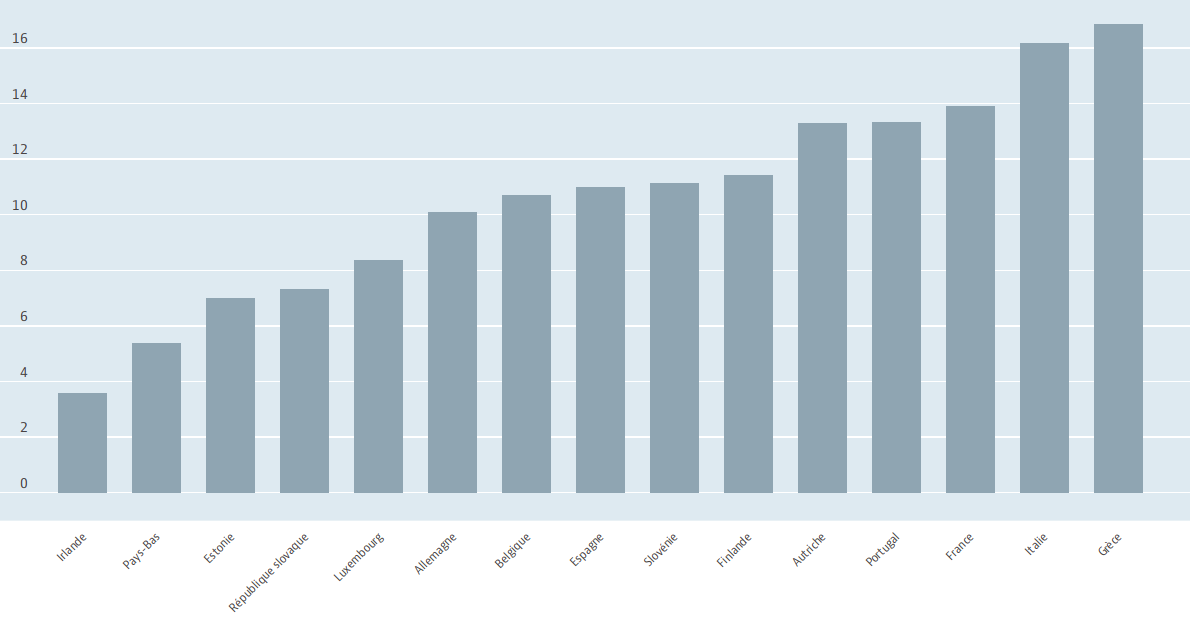
\includegraphics[width=0.95\textwidth]{Depenses-retraites-2015-UE-15.png}
\end{center}
\caption{Dépenses de retraite publiques en \% du PIB en 2015 de 15 pays de la zone Euro. 
OCDE (2020). }
\label{fig-depenses-UE-15-2020}
\end{figure}

Pour obtenir une valeur de référence en 2070, nous pouvons projetter les dépenses de 
retraites dans le futur dans d'autres pays de l'union européenne.  
La figure \ref{fig-depenses-France-Allemagne} extraite 
d'un rapport au Sénat de 2011 par Bernard Angels présente une analyse 
comparée du montant des dépenses en France et en Allemagne en 2060. 
Ces estimations réalisées en 2009 ne tiennent pas compte des réformes, 
notamment celles des retraites, adoptées depuis. 
On observe que le montant des dépenses de retraites prévues en 2060 
en Union Européenne des 27 est de 12.5 \% de PIB.

\begin{figure}
\begin{center}
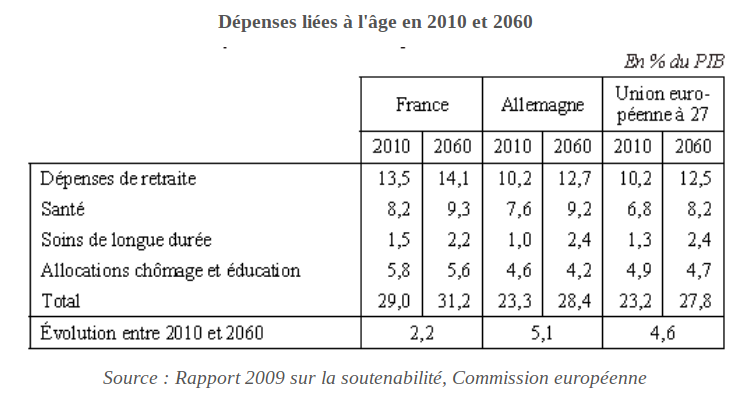
\includegraphics[width=0.7\textwidth]{Depenses-retraites-2010-2060-France-Allemagne.png}
\end{center}
\caption{}
\label{fig-depenses-France-Allemagne}
\end{figure}

La trajectoire de dépenses que nous considérons consiste à utiliser les mêmes 
niveaux de dépenses que l'étude d'impact de 2020 à 2050. 
Pour la période 2050-2070, nous faisons l'hypothèse que le niveau 
de dépense s'abaisse jusqu'à 12,6 \% du PIB en 2070. 
Nous utilisons pour cela une interpolation de degré 2 fondée sur une spline. 
Cette méthode permet d'assurer la continuité de la trajectoire ainsi que la continuité 
de la dérivée première. 
L'hypothèse générale de cette trajectoire est que le montant des dépenses 
va baisser en direction de la moyenne européenne. 
La valeur numérique que nous avons retenue, c'est à dire 12.6\%, est fondée premièrement 
sur le fait que ce montant est mentionné dans l'étude d'impact, même si celui-ci ne peut pas 
être considéré comme un montant exactement comparable puisqu'il porte 
sur un périmètre plus "large que les dépenses du seul système de retraite". 
C'est pourquoi, nous avons considéré que c'est une hypothèse plutôt optimiste. 
La figure \ref{fig-dépenses-simulation} présente le résultat. 

\begin{figure}
\begin{center}
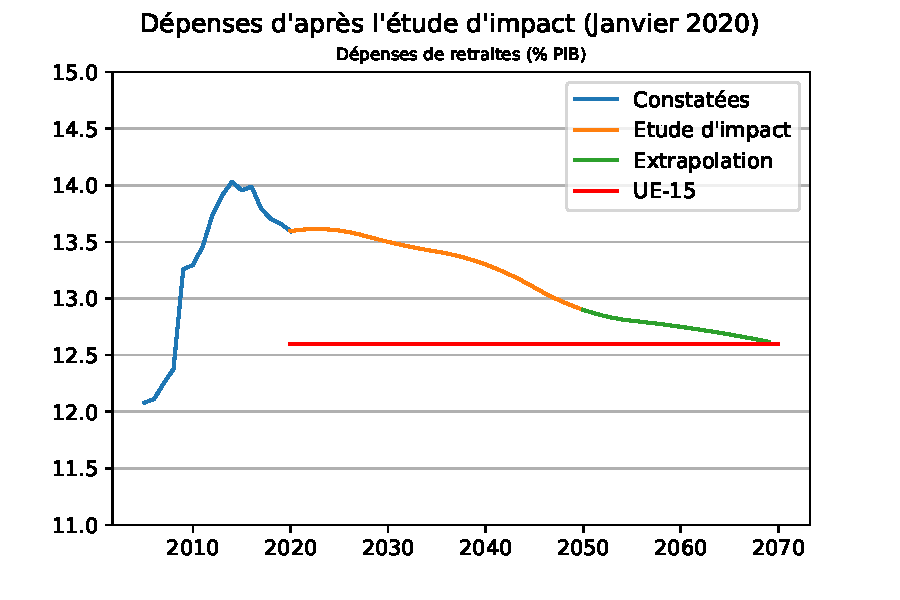
\includegraphics[width=0.7\textwidth]{Simulation-Depenses.pdf}
\end{center}
\caption{Dépenses dans notre simulation de l'étude d'impact.}
\label{fig-dépenses-simulation}
\end{figure}

%%%%%%%%%%%%%%%%%%%%%%%%%%%%%%%%%%%%%%%%%%%%%%

\subsection{L'âge de départ en retraite}

Reproduire l'âge de départ en retraite dans notre simulation 
pose des difficultés. 

Le graphique 49 page 139 de l'étude d'impact de Janvier 2020 est présenté 
dans la figure \ref{fig-age-etude-impact}.

\begin{figure}
\begin{center}
\includegraphics[width=0.9\textwidth]{../Figures-Etude-Impact/EtudeImpact-Graphique-49-AgeDepartRetraite.png}
\end{center}
\caption{Age de départ à la retraite dans le graphique 49 de l'étude d'impact.}
\label{fig-age-etude-impact}
\end{figure}

Le texte précise : "Au total, en tenant compte de l’ensemble de ces 
décalages, l’âge moyen de départ serait plus élevé dans le système 
universel : 64 ans et 5 mois contre 64 ans et 10 mois environ dans 
le système actuel pour la génération 1990." 
Remarquons que le texte semble comporter une coquille, avec une inversion 
des âges dans les deux systèmes : l'aĝe dans le système universel sera supérieur, 
bien sûr ! 

Le graphique 73 page 199 de l'étude d'impact de Janvier 2020 est présenté 
dans la figure \ref{fig-age-etude-impact-graphique-73}.

\begin{figure}
\begin{center}
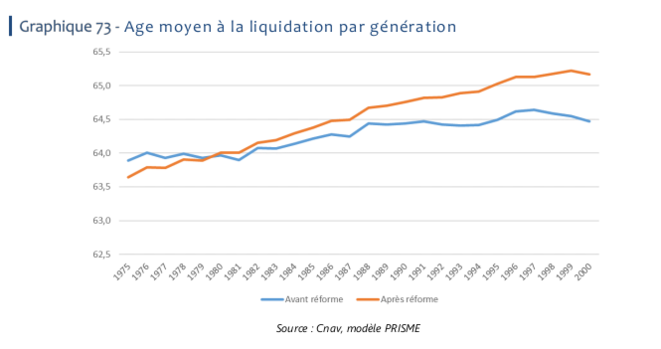
\includegraphics[width=0.9\textwidth]{../Figures-Etude-Impact/EtudeImpact-Graphique-73-AgeDepartRetraite.png}
\end{center}
\caption{Age de départ à la retraite dans le graphique 73 de l'étude d'impact.}
\label{fig-age-etude-impact-graphique-73}
\end{figure}

Le texte précise : "La hausse de l’âge moyen de liquidation permet d’augmenter 
significativement les pensions versées : la prise en compte des comportements 
augmente ainsi la pension moyenne de 5 \% pour la génération 1990."

Sur le graphique 73 de l'étude d'impact, nous lisons les valeurs numériques 
suivantes après réforme :
\begin{itemize}
\item un âge de départ à 63,6 ans pour la génération 1975,
\item un âge de départ à 65,2 ans pour la génération 2000.
\end{itemize}

On observe que la génération 1975 partira en retraite en 2038 dans le scénario de l'étude d'impact puisque 1975 + 63,6 = 2038.6.
Remarquons que l'horizon temporel de cette partie de l'étude d'impact est l'année 2065, puisque 2000 + 65,2 = 2065.2. 
Ce choix peut sembler pour le moins \emph{étonnant}, dans la mesure où cet horizon 
est l'année 2050 pour d'autres aspects de l'étude d'impact, 
comme par exemple la trajectoire de dépenses du tableau 39. 

Pour calculer l'âge de départ en retraite en fonction de l'année du départ, 
nous réalisons une inversion mathématique.  

Notre calcul se décompose en trois parties :
\begin{itemize}
\item jusqu'à l'année 2039 (année du départ à la retraite 
de la génération 1975), nous utilisons les données du COR, 
\item de 2039 à 2065 (année du départ à la retraite de la génération 
2000), nous utilisons les données de l'étude d'impact,
\item de 2065 à 2070, nous extrapolons. 
\end{itemize}


Le résultat de notre simulation est présenté dans la figure \ref{fig-simulation-A}. 

\begin{figure}
\begin{center}
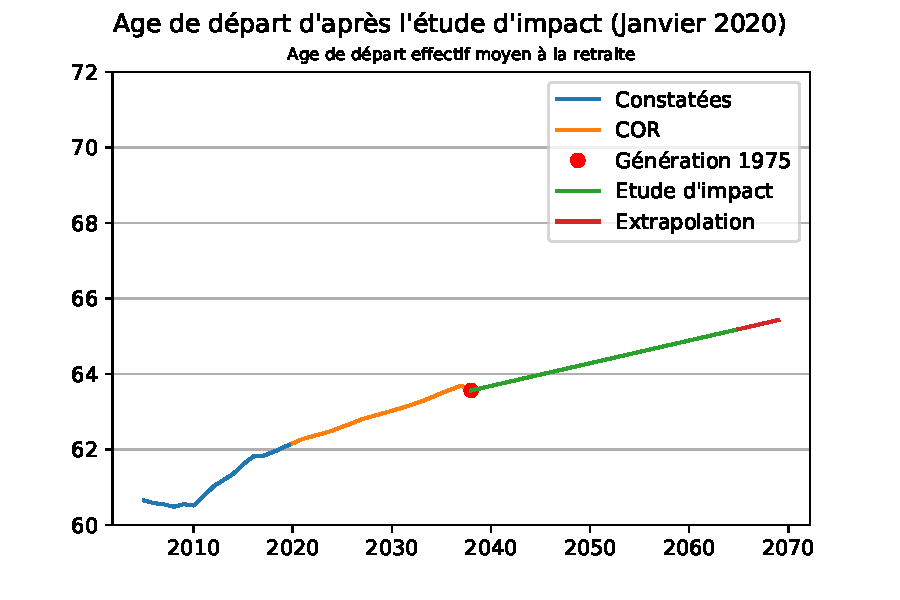
\includegraphics[width=0.7\textwidth]{Simulation-Age.pdf}
\end{center}
\caption{L'âge de départ en retraite moyen dans notre simulation.}
\label{fig-simulation-A}
\end{figure}

La trajectoire de l'âge de départ en retraite est discontinue car l'âge prévu par le COR en 2038 n'est pas égal à celui que nous avons inféré depuis le graphique 73. Dans l'étude d'impact, nous avons utilisé un âge de départ à la retraite égal à 63,6 alors qu'un âge permettant d'assurer la continuité serait égal à 63,8.

Nous avons calculé l'âge de départ en retraite moyen pour l'ensemble des retraités partant en retraite en 2038 en fonction seulement de l'âge de départ en retraite de la génération 1975. Notre calcul n'est donc qu'une approximation, puisque les personnes partant en retraite en 2038 ne sont pas toutes de la génération 1975. L'étude d'impact ne donnant pas d'information sur l'âge moyen de départ en retraite en 2038, il ne semble pas facile de faire un calcul plus précis. 

%%%%%%%%%%%%%%%%%%%%%%%%%%%%%%%%%%%%%%%%%%%%%%

\section{Résultats}

\subsection{Effets de la réforme}

Dans ce paragraphe, nous étudions les effets de la réforme Macron-Philippe dans 
le scénario central d'un taux de chômage égal à 7\% 
et d'un taux de hausse des salaires égal à +1.3\%. 
La trajectoire avant réforme est celle du COR et la trajectoire après réforme est celle 
que nous avons calculé avec notre simulateur dans le but de reproduire les 
résultats de l'étude d'impact. 

Dans la figure \ref{fig-solde-avant-apres-reforme}, nous présentons le 
solde financier avant et après réforme. 
On observe que après réforme, le solde est rigoureusement nul, 
alors que, avant réforme, le solde peut être négatif dans ce scénario. 

\begin{figure}
\begin{center}
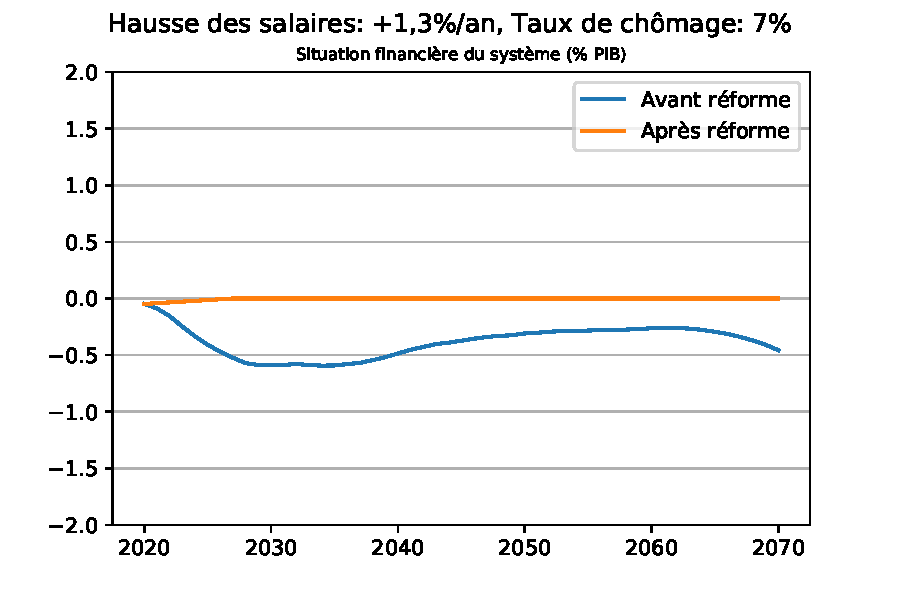
\includegraphics[width=0.7\textwidth]{Simulation-vs-avant-reforme-Solde.pdf}
\end{center}
\caption{Solde financier avant et après réforme.}
\label{fig-solde-avant-apres-reforme}
\end{figure}

Dans la figure \ref{fig-depenses-avant-apres-reforme}, nous présentons les 
dépenses de retraites avant et après réforme. 
On observe que après réforme, les dépenses sont inférieures à ce qu'elles 
étaient avant réforme. 

\begin{figure}
\begin{center}
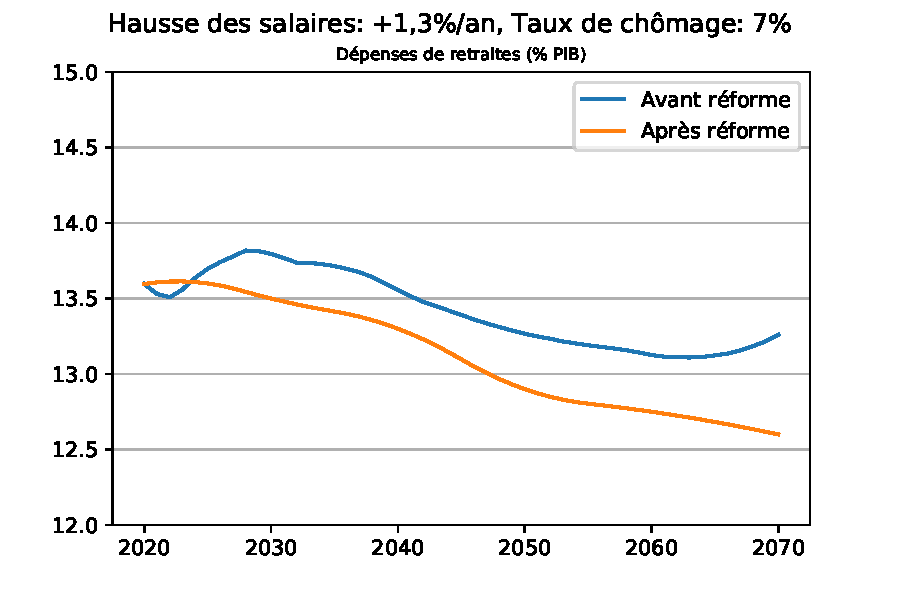
\includegraphics[width=0.7\textwidth]{Simulation-vs-avant-reforme-Depenses.pdf}
\end{center}
\caption{Dépenses de retraite avant et après réforme.}
\label{fig-depenses-avant-apres-reforme}
\end{figure}

La figure \ref{fig-simulation-A-vs-COR} compare l'âge effectif moyen 
de départ à la retraite avant et après réforme. 
On observe que l'âge de départ à la retraite est donc 
significativement supérieur dans l'étude d'impact comparé au calcul du COR de Juin 2019. 
Notre extrapolation a mené à un âge de départ à la retraite égal à 
environ 65.5 ans en 2070. 
Nous ne savons pas si cet âge est réaliste, mais nous notons deux éléments. 
\begin{itemize}
\item Le COR prévoyait une augmentation de l'âge de départ moins 
forte à partir de 2040. 
\item Si l'âge réel de départ à la retraite ne suit pas la courbe 
que nous avons imposée, alors les pensions de retraites que nous 
obtiendrons en conséquence seront inférieures à celles que nous avons 
simulées. 
\end{itemize}

\begin{figure}
\begin{center}
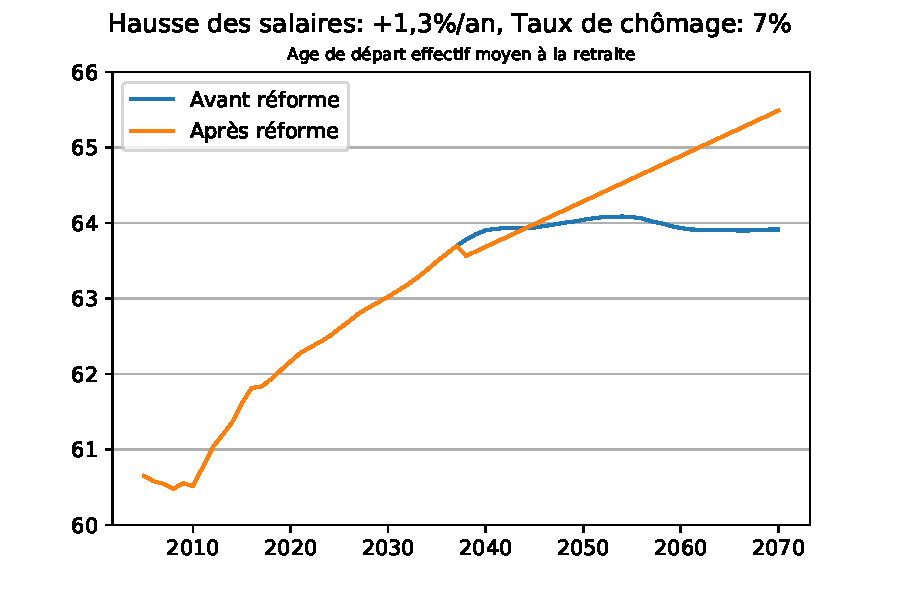
\includegraphics[width=0.7\textwidth]{Simulation-vs-avant-reforme-Age.pdf}
\end{center}
\caption{L'âge de départ en retraite moyen dans l'étude d'impact comparé 
au calcul du COR.}
\label{fig-simulation-A-vs-COR}
\end{figure}


%%%%%%%%%%%%%%%%%%%%%%%%%%%%%%%%%%%%%%%%%%%%%%

\subsection{Le niveau des pensions par rapport aux actifs}

La figure \ref{fig-simulation-P} présente le rapport entre la pension moyenne et le salaire moyen. 

\begin{figure}
\begin{center}
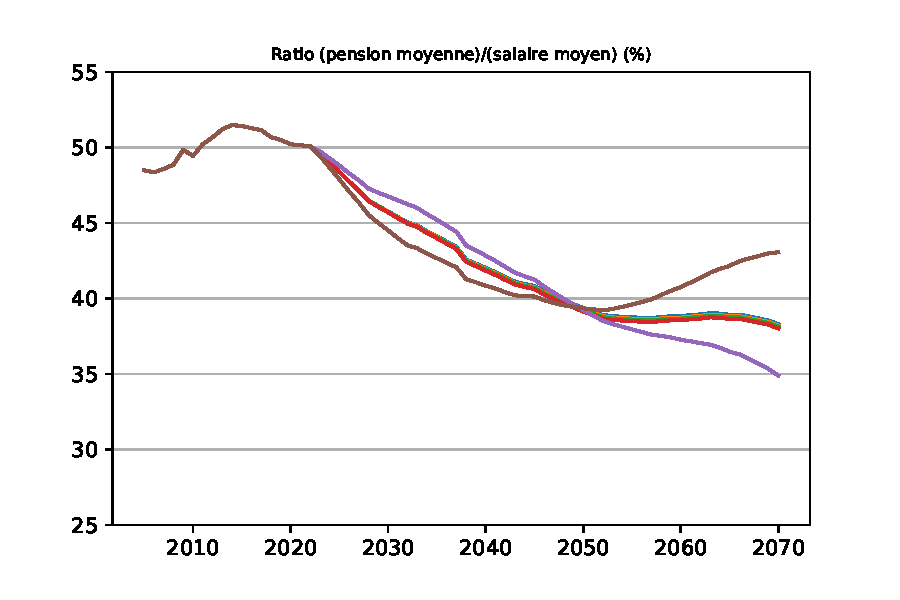
\includegraphics[width=0.8\textwidth]{Simulation-P.pdf}

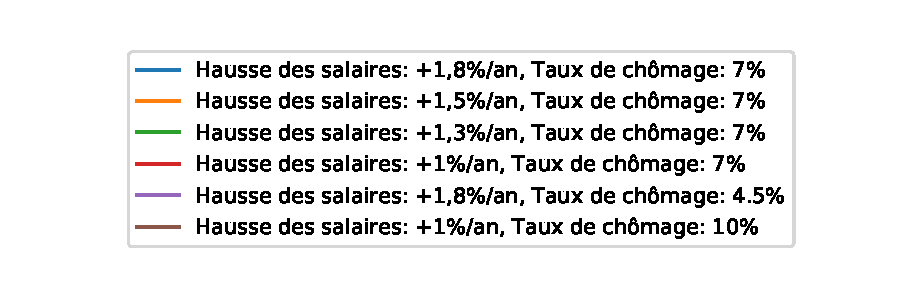
\includegraphics[width=0.7\textwidth]{Simulation-legende.pdf}
\end{center}

\caption{Le niveau de pensions par rapport aux actifs après réforme 
d'après notre simulation, avec les hypothèses de l'étude d'impact.}
\label{fig-simulation-P}
\end{figure}

Pour les quatre scénarios principaux (associés au taux de chômage 
de 7\%), on observe que le niveau des pensions par rapport aux actifs 
baisse de 50\% en 2020 jusqu'en 2050 autour de 39\%, puis se stabilise ensuite. 
Relativement au niveau actuel de ce ratio, la baisse est donc d'environ 20\%. 

On observe que le niveau de pensions n'est pas très sensible 
aux taux de hausse des salaires, puisque les quatre courbes associées 
à +1\%, +1.3\%, +1.5\%,  +1.8\% sont très proches. 
En revanche, le niveau des pensions est très sensible au taux de chômage : 
un taux de chômage élevé et égal à 10\% (dans le scénario pessimiste) 
fait remonter le niveau des pensions à près de 44\% tandis qu'un taux de 
chômage faible et égal à 4.5\% (dans le scénario optimiste) fait baisser 
le niveau à près de 36\%. 

Page 80 de l'étude d'impact, le texte indique que la réforme 
réduit "l’exposition du système aux fluctuations économiques et démographiques". 
On constate que c'est faux, dans la mesure où le niveau des pensions 
dépend fortement du taux de chômage.

La figure \ref{fig-simulation-P-vs-COR} compare le niveau des pensions par rapport 
aux salaires avant et après réforme. 

\begin{figure}
\begin{center}
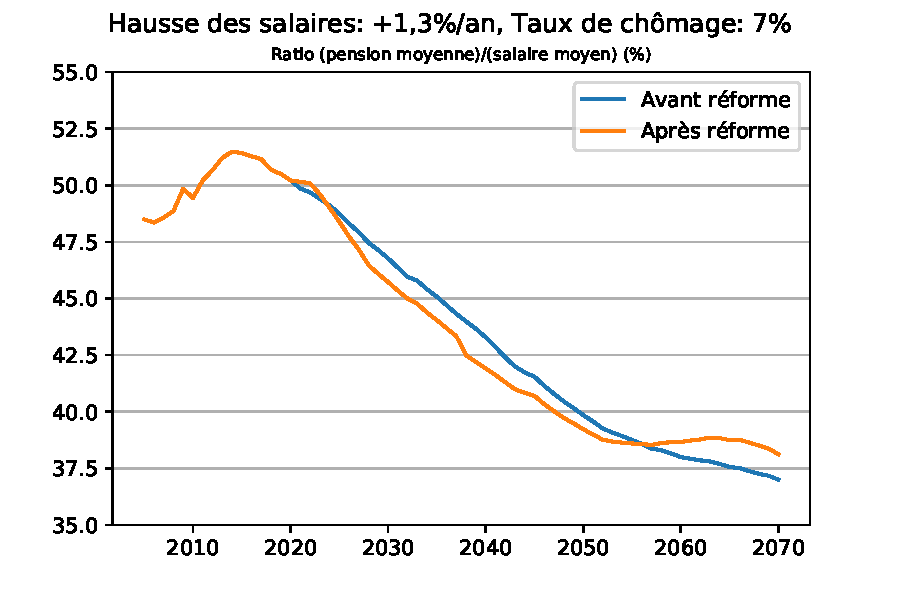
\includegraphics[width=0.7\textwidth]{Simulation-vs-avant-reforme-Pensions.pdf}
\end{center}
\caption{Le niveau des pensions par rapport aux salaires 
avant et après réforme.}
\label{fig-simulation-P-vs-COR}
\end{figure}

%%%%%%%%%%%%%%%%%%%%%%%%%%%%%%%%%%%%%%%%%%%%%%

\subsection{Le niveau absolu des pensions dans l'étude d'impact}

Le lecteur de l'étude d'impact sera très étonné à la lecture de la figure 
\ref{fig-simulation-P}. 
En effet, à la page 176 de l'étude d'impact, le graphique 59, 
reproduit dans la figure \ref{fig-pension-annuelle-etude-impact}, 
présente une pension annuelle moyenne plutôt favorable au système 
universel.
Le texte précise : "En moyenne, les niveaux des pensions servies augmentent 
avec la mise en place du système universel."

\begin{figure}
\begin{center}
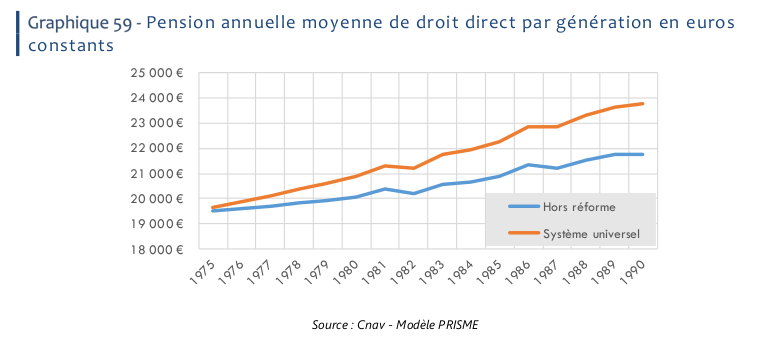
\includegraphics[width=0.9\textwidth]{../Figures-Etude-Impact/EtudeImpact-Graphique-59-PensionAnnuelle.png}
\end{center}

\caption{Pension annuelle moyenne dans l'étude d'impact.}
\label{fig-pension-annuelle-etude-impact}
\end{figure}

Deux éléments sont significatifs dans le graphique 59. 
Premièrement, la vitesse de croissance de la pension annuelle est forte. 
Deuxièmement, la réforme améliore significativement la pension annuelle 
par rapport à la situation hors réforme. 

Pour évaluer la pension annuelle moyenne de droit direct, on ne peut pas, 
une fois de plus, utiliser le simulateur du COR car
il ne fournit pas ce résultat.
C'est pourquoi nous avons utilisé notre simulateur en ajoutant les équations 
nécessaires. 
Nous avons obtenu la figure \ref{fig-pension-annuelle-simulation} qui présente 
la pension annuelle moyenne de droit direct avec les hypothèses de l'étude d'impact. 

\begin{figure}
\begin{center}
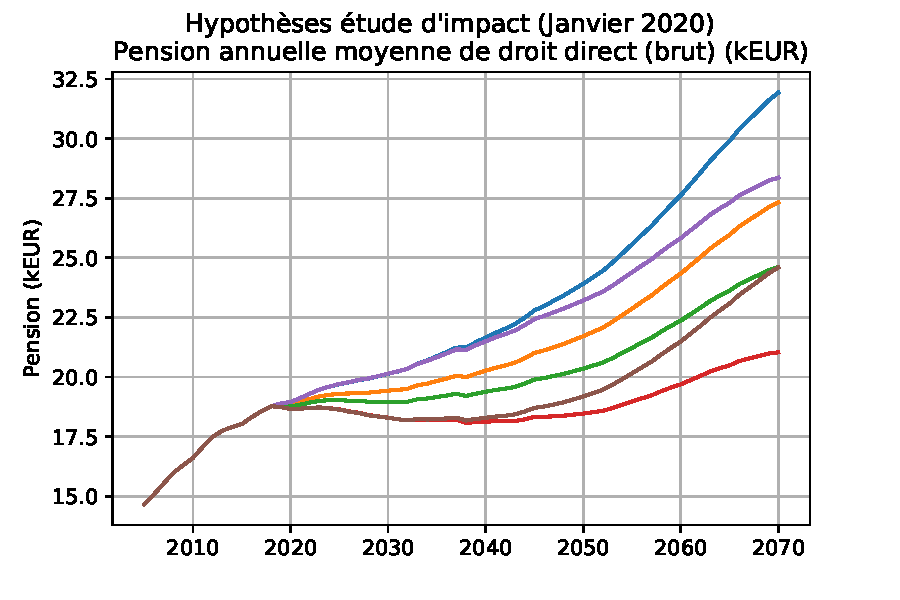
\includegraphics[width=0.7\textwidth]{Simulation-pension-annuelle-moyenne.pdf}

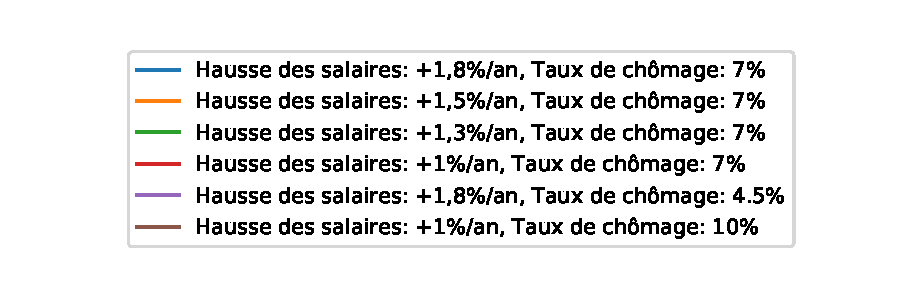
\includegraphics[width=0.7\textwidth]{Simulation-legende.pdf}
\end{center}

\caption{Pension annuelle moyenne d'après notre simulation 
avec les hypothèses de l'étude d'impact.}
\label{fig-pension-annuelle-simulation}
\end{figure}

On observe que la pension annuelle moyenne augmente dans le scénario central de 
l'étude d'impact (hausse des salaires : +1.3\%, taux de chômage : 7\%). 
Toutefois, on observe que la vitesse de cette augmentation est moins importante 
que dans le graphique 59 de l'étude d'impact. 
De plus, on observe que les pensions peuvent temporairement baisser dans certains 
des scénarios économiques, comme lorsque la hausse des salaires n'est que 
de +1\%. 

La figure \ref{fig-pension-annuelle-simulation-vs-COR} présente la pension 
annuelle moyenne brut avec et sans réforme. 
Nous observons que les montants sont similaires: la réforme ne présente donc pas 
d'avantage de ce point de vue. 

\begin{figure}
\begin{center}
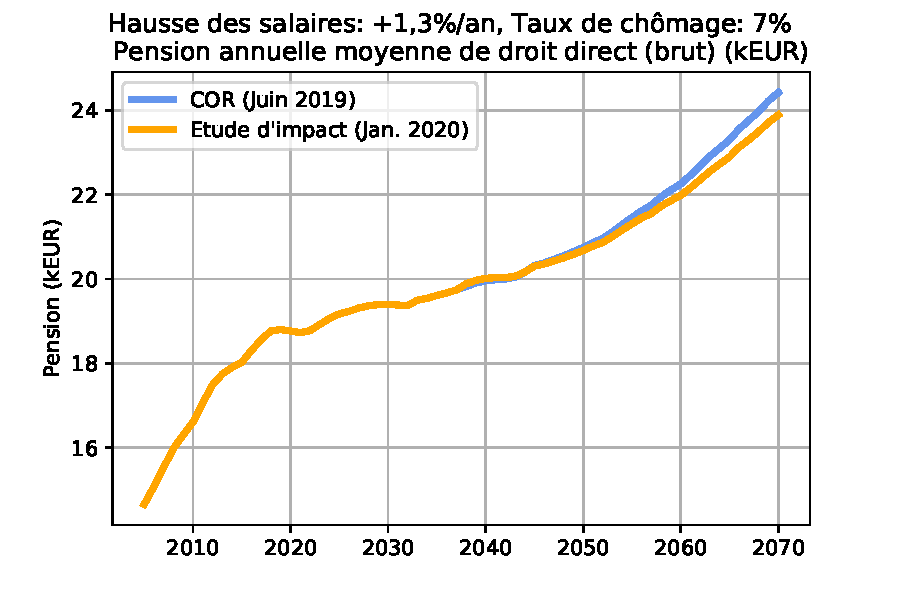
\includegraphics[width=0.7\textwidth]{Simulation-pension-annuelle-moyenne-3.pdf}
\end{center}
\caption{Pension annuelle moyenne dans le scénario central 
avant et après réforme.}
\label{fig-pension-annuelle-simulation-vs-COR}
\end{figure}

La figure \ref{fig-pension-annuelle-avant-apres-salaires} présente la pension 
annuelle moyenne brut avec et sans réforme, comparé aux salaires. 
Il n'est pas possible, en toute rigueur, de comparer des salaires et 
des pensions en valeur absolue, puisque les pensions sont inférieures aux 
salaires. 
C'est pourquoi nous avons rapporté ces montants absolus à une base 100 en 2020.  
On observe que, sur la période 2020-2070, les salaires augmentent de plus de 80\% 
alors que les pensions annuelles brutes n'augmentent que de 30\%. 

\begin{figure}
\begin{center}
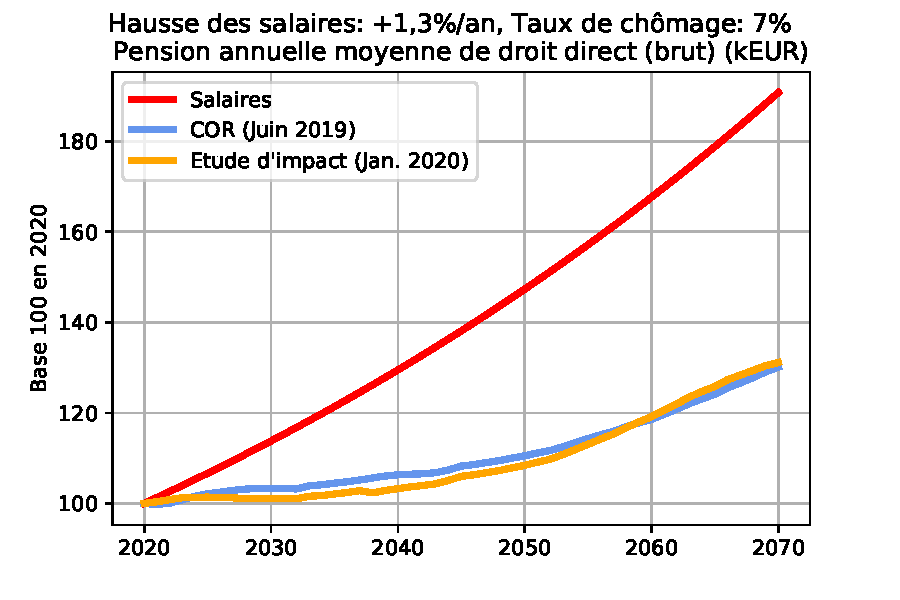
\includegraphics[width=0.7\textwidth]{Simulation-pension-vs-salaires-3.pdf}
\end{center}
\caption{Pension annuelle moyenne dans le scénario central 
avant et après réforme, comparé aux salaires.}
\label{fig-pension-annuelle-avant-apres-salaires}
\end{figure}

Ainsi, en changeant d'indicateur, l'étude d'impact peut montrer une situation 
dont l'apparence est favorable. 

%%%%%%%%%%%%%%%%%%%%%%%%%%%%%%%%%%%%%%%%%%%%%%

\subsection{Et si l'âge moyen de départ était modifié ?}

On peut se demander ce qui pourrait 
advenir en conservant la règle d'équilibre financière et le niveau de dépenses actuel
mais en laissant varier l'âge de départ à la retraite. 
En effet, on peut penser que l'âge prévu par la réforme actuelle 
ne sera pas atteint car trop élevé. 
Les salariés ne pourront donc pas tous liquider leur retraite au moment
supposé jusqu'ici. 
Au contraire, suite à une remarquable amélioration des conditions de vie, 
l'âge de départ à la retraite pourrait être repoussé au delà de ce qui 
était initialement prévu. 

La figure \ref{fig-simulation-age-vs-pensions} présente, pour une année future donnée, 
l'ensemble des niveaux de pensions par rapport aux salaires qui peuvent être atteints avec 
un âge de départ à la retraite donné. 

\begin{figure}
\begin{center}
\includegraphics[width=0.7\textwidth]{Simulation-Age-vs-pensions-vs-date.pdf}
\end{center}

\caption{Le niveau de pensions en fonction de l'âge et de l'année.}
\label{fig-simulation-age-vs-pensions}
\end{figure}

En 2020, l'âge de départ à la retraite égal à 62 ans 
mène à un rapport pensions/salaire égal à 0.5 (situation actuelle).  
En 2055, si l'âge de départ est maintenu à 62 ans, alors ce ratio baisse jusqu'à 0.32, 
une situation très défavorable pour les retraités futurs
Au contraire, si en 2055 l'âge de départ est repoussé à 69 ans, 
alors le ratio est égal à 0.5. 
Il reste que cet âge de départ semble hypothétique, au vu de l'âge de départ actuel. 
% Suggestion : ajouter la trajectoire prévue dans l'étude d'impact

%%%%%%%%%%%%%%%%%%%%%%%%%%%%%%%%%%%%%%%%%%%%%%

\section{Conclusion}

Nous avons vu comment la logique du projet de loi est une 
rupture dans le pilotage du système de retraites, 
imposant l'équilibre financier et le volume des dépenses 
à priori : en fonction de l'âge de départ à la retraite, 
les pensions devront donc s'ajuster \emph{en conséquence}. 
De plus, nous avons observé ce qui nous était caché dans l'étude 
d'impact, c'est à dire ce qui se passe entre 2050 et 2070 ainsi que 
la sensibilité du niveau de pension en fonction des scénarios 
de conjoncture. 
Nous avons vu comment le montant des dépenses de retraites avec la réforme 
des retraites est en baisse par rapport au niveau actuel. 
Enfin, nous avons vu comment la réforme est fallacieusement 
montrée comme avantageuse du point de vue du montant des pensions. 

Les citoyens que nous sommes peuvent comprendre qu'une proposition de loi 
aille dans un sens politique que nous ne partageons pas : c'est le 
fonctionnement actuel de la République. 
En revanche, nous ne pouvons pas accepter que la décision politique soit 
prise en fonction de données qui ne sont pas ouvertes, 
de calculs qui ne sont pas publics et, finalement, sur la base d'études trompeuses. 

%%%%%%%%%%%%%%%%%%%%%%%%%%%%%%%%%%%%%%%%%%%%%%

\section{Annexe}

Pour les lecteurs désirant reproduire les simulations de ce texte, 
nous présentons ci-dessous les paramètres que nous avons calculés dans 
le scénario hausse des salaires: +1,3 \%/an, taux de chômage: 7\%.

\begin{center}
\begin{tabular}{l|lll}
\textbf{Année} & \textbf{Age} & \textbf{Cotis.} & \textbf{Pension} \\
\hline
 2020 & 62.2 ans & 30.8 \% & 50.2 \% \\
 2025 & 62.6 ans & 30.9 \% & 48.4 \% \\
 2030 & 63.0 ans & 30.7 \% & 45.7 \% \\
 2040 & 63.9 ans & 30.2 \% & 42.4 \% \\
 2050 & 64.5 ans & 29.3 \% & 39.7 \% \\
 2060 & 65.2 ans & 28.8 \% & 39.0 \% \\
 2070 & 65.8 ans & 28.6 \% & 38.8 \%
\end{tabular}
\end{center}

Pour tester graphiquement les effets de ces paramètres, nous vous recommandons le 
simulateur du collectifs "Nos retraites" \url{https://nosretraites.github.io/roc-retraites}. 

%%%%%%%%%%%%%%%%%%%%%%%%%%%%%%%%%%%%%%%%%%%%%%

\section{Références}

\begin{itemize}
\item Projet de loi instituant un système universel de retraite. - Etude d'impact, 24 janvier 2020
\item Évolutions et perspectives des retraites en France. Rapport annuel du COR – Juin 2019
\item \url{https://www.cor-retraites.fr/simulateur}
\item Simulateur du COR / Documentation technique - juillet 2016
\item \url{https://github.com/brunoscherrer/retraites}
\item \url{https://nosretraites.github.io/roc-retraites/}
\item Prospective du couple franco-allemand
Repères. 22 juin 2011. 
Prospective du couple franco-allemand (rapport d'information). 
Bernard ANGELS, Rapport d'information numéro 663.
\end{itemize}

%%%%%%%%%%%%%%%%%%%%%%%%%%%%%%%%%%%%%%%%%%%%%%

\section{Remerciements}

Nous remercions chaleureusement Michaël Zemmour pour son support 
technique et ses encouragements dans la réalisation de cet article. 
Nous remercions Joseph Muré pour son travail de relecture. 

%%%%%%%%%%%%%%%%%%%%%%%%%%%%%%%%%%%%%%%%%%%%%%

\section{Annexes}

\subsection{Le niveau de vie des retraités par rapport à l'ensemble de la population}

La figure \ref{fig-simulation-RNV-vs-pensions} présente 
le niveau de vie des retraités par rapport aux actifs. 
D'après la documentation technique du COR : "Le niveau de vie est défini 
par l’INSEE, au niveau de chaque ménage, comme le revenu disponible (tenant
compte de l’ensemble des ressources et après prélèvements et transferts sociaux) 
divisé par le nombre d’unités de consommation dans le ménage 
(qui dépend du nombre de personnes qui le composent, cf. page 4)."

\begin{figure}
\begin{center}
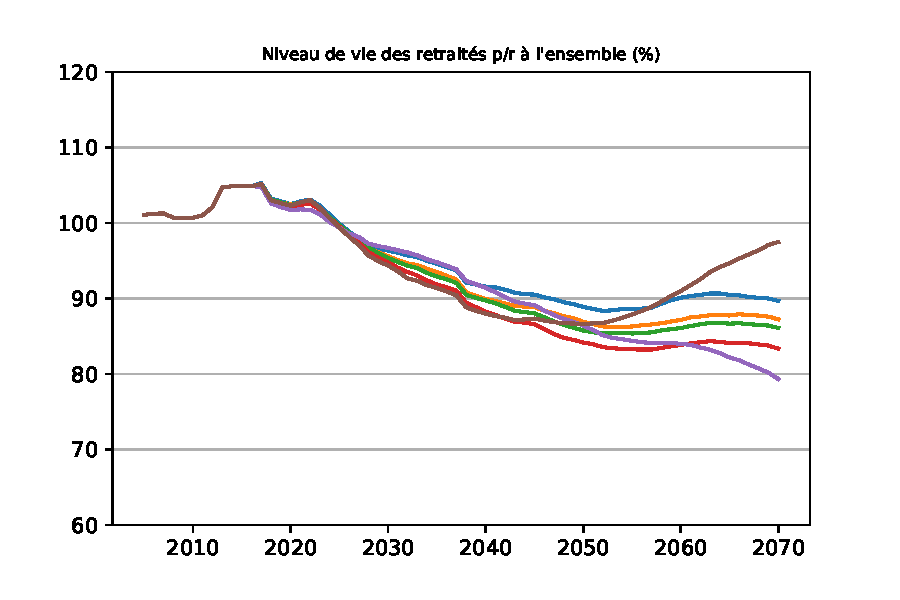
\includegraphics[width=0.8\textwidth]{Simulation-RNV.pdf}

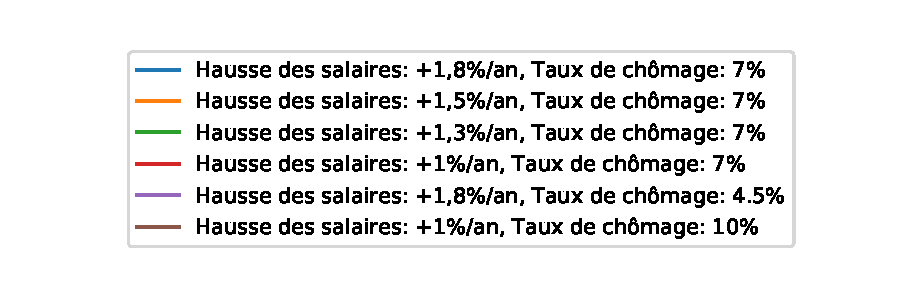
\includegraphics[width=0.6\textwidth]{Simulation-legende.pdf}
\end{center}

\caption{Le niveau de pensions en fonction de l'âge et de l'année.}
\label{fig-simulation-RNV-vs-pensions}
\end{figure}

On observe que le niveau de vie des retraités 
baisse de 105\% en 2020 jusqu'en 2050 entre 85\% et 90\%, puis se stabilise ensuite. 

\end{document}
